Subbab-subbab sebelumnya telah menyajikan hasil uji Mann-Whitney U untuk
setiap metrik secara terpisah: minimum clearance pada
Subbab~\ref{sec:analisis_keselamatan}, waktu tempuh, panjang lintasan, dan
kecepatan linear pada Subbab~\ref{sec:tradeoff}, serta kecepatan angular
pada Subbab~\ref{sec:kehalusan_gerak}. Interpretasi berdasarkan nilai $p$
saja sudah cukup untuk menyatakan ada atau tidaknya perbedaan distribusi,
namun belum menjawab seberapa besar perbedaan itu berarti secara praktis.
Subbab ini menyatukan seluruh hasil tersebut, dengan effect size sebagai
pelengkap wajib pada setiap kesimpulan signifikansi, sebagai dasar bagi
pembahasan terintegrasi pada Subbab 4.8.

\begin{table}[H]
\centering
\caption{Rekapitulasi hasil uji Mann-Whitney U untuk seluruh metrik kontinu
pada keempat pasangan skenario ($\alpha=0,05$).}
\label{tab:rekap_mwu}
\begin{tabular}{llccc}
\toprule
\textbf{Metrik} & \textbf{Pasangan} & \textbf{$U$} & \textbf{$p$} & \textbf{Signifikan} \\
\midrule
\multirow{4}{*}{Minimum Clearance (m)}
 & S1--S5 & n/a & n/a    & n/a \\
 & S2--S6 & 10  & 0,0013 & **  \\
 & S3--S7 & 0   & 0,0002 & *** \\
 & S4--S8 & 0   & 0,0002 & *** \\
\midrule
\multirow{4}{*}{Waktu Tempuh (s)}
 & S1--S5 & 0  & 0,0002 & *** \\
 & S2--S6 & 20 & 0,0257 & *  \\
 & S3--S7 & 0  & 0,0002 & *** \\
 & S4--S8 & 0  & 0,0002 & *** \\
\midrule
\multirow{4}{*}{Panjang Lintasan (m)}
 & S1--S5 & 79 & 0,0243 & *  \\
 & S2--S6 & 20 & 0,0254 & *  \\
 & S3--S7 & 0  & 0,0002 & *** \\
 & S4--S8 & 4  & 0,0006 & *** \\
\midrule
\multirow{4}{*}{Kecepatan Linear (m/s)}
 & S1--S5 & 100 & 0,0002 & *** \\
 & S2--S6 & 80  & 0,0251 & *  \\
 & S3--S7 & 100 & 0,0002 & *** \\
 & S4--S8 & 99  & 0,0002 & *** \\
\midrule
\multirow{4}{*}{Kecepatan Angular (rad/s)}
 & S1--S5 & 100 & 0,0002 & *** \\
 & S2--S6 & 100 & 0,0002 & *** \\
 & S3--S7 & 6   & 0,0009 & *** \\
 & S4--S8 & 38  & 0,4055 & ns  \\
\bottomrule
\end{tabular}
\end{table}

\begin{table}[H]
\centering
\caption{Rekapitulasi effect size (\textit{rank-biserial correlation})
untuk seluruh metrik kontinu pada keempat pasangan skenario.}
\label{tab:rekap_effect_size}
\begin{tabular}{llcc}
\toprule
\textbf{Metrik} & \textbf{Pasangan} & \textbf{Effect Size ($r$)} & \textbf{Interpretasi} \\
\midrule
\multirow{4}{*}{Minimum Clearance}
 & S1--S5 & n/a   & n/a \\
 & S2--S6 & +0,80 & Besar \\
 & S3--S7 & +1,00 & Besar \\
 & S4--S8 & +1,00 & Besar \\
\midrule
\multirow{4}{*}{Waktu Tempuh}
 & S1--S5 & +1,00 & Besar \\
 & S2--S6 & +0,60 & Besar \\
 & S3--S7 & +1,00 & Besar \\
 & S4--S8 & +1,00 & Besar \\
\midrule
\multirow{4}{*}{Panjang Lintasan}
 & S1--S5 & -0,58 & Besar \\
 & S2--S6 & +0,60 & Besar \\
 & S3--S7 & +1,00 & Besar \\
 & S4--S8 & +0,92 & Besar \\
\midrule
\multirow{4}{*}{Kecepatan Linear}
 & S1--S5 & -1,00 & Besar \\
 & S2--S6 & -0,60 & Besar \\
 & S3--S7 & -1,00 & Besar \\
 & S4--S8 & -0,99 & Besar \\
\midrule
\multirow{4}{*}{Kecepatan Angular}
 & S1--S5 & -1,00 & Besar \\
 & S2--S6 & -1,00 & Besar \\
 & S3--S7 & +0,88 & Besar \\
 & S4--S8 & +0,23 & Kecil \\
\bottomrule
\end{tabular}
\end{table}

Dari 20 kombinasi metrik-pasangan pada Tabel~\ref{tab:rekap_mwu}, 19
kombinasi dapat diuji secara statistik (satu kombinasi, minimum clearance
pada S1/S5, tidak dapat diuji karena kedua kelompok konstan dan identik,
sebagaimana telah dijelaskan pada Subbab~\ref{sec:analisis_keselamatan}).
Dari 19 kombinasi yang diuji, 18 signifikan pada $\alpha=0,05$, dan seluruh
18 kombinasi tersebut tergolong effect size besar pada
Tabel~\ref{tab:rekap_effect_size}. Satu-satunya kombinasi yang tidak
signifikan pada keseluruhan penelitian ini adalah kecepatan angular pada
S4/S8 ($p=0,4055$; $r=+0,23$, kategori kecil).

\begin{figure}[H]
\centering
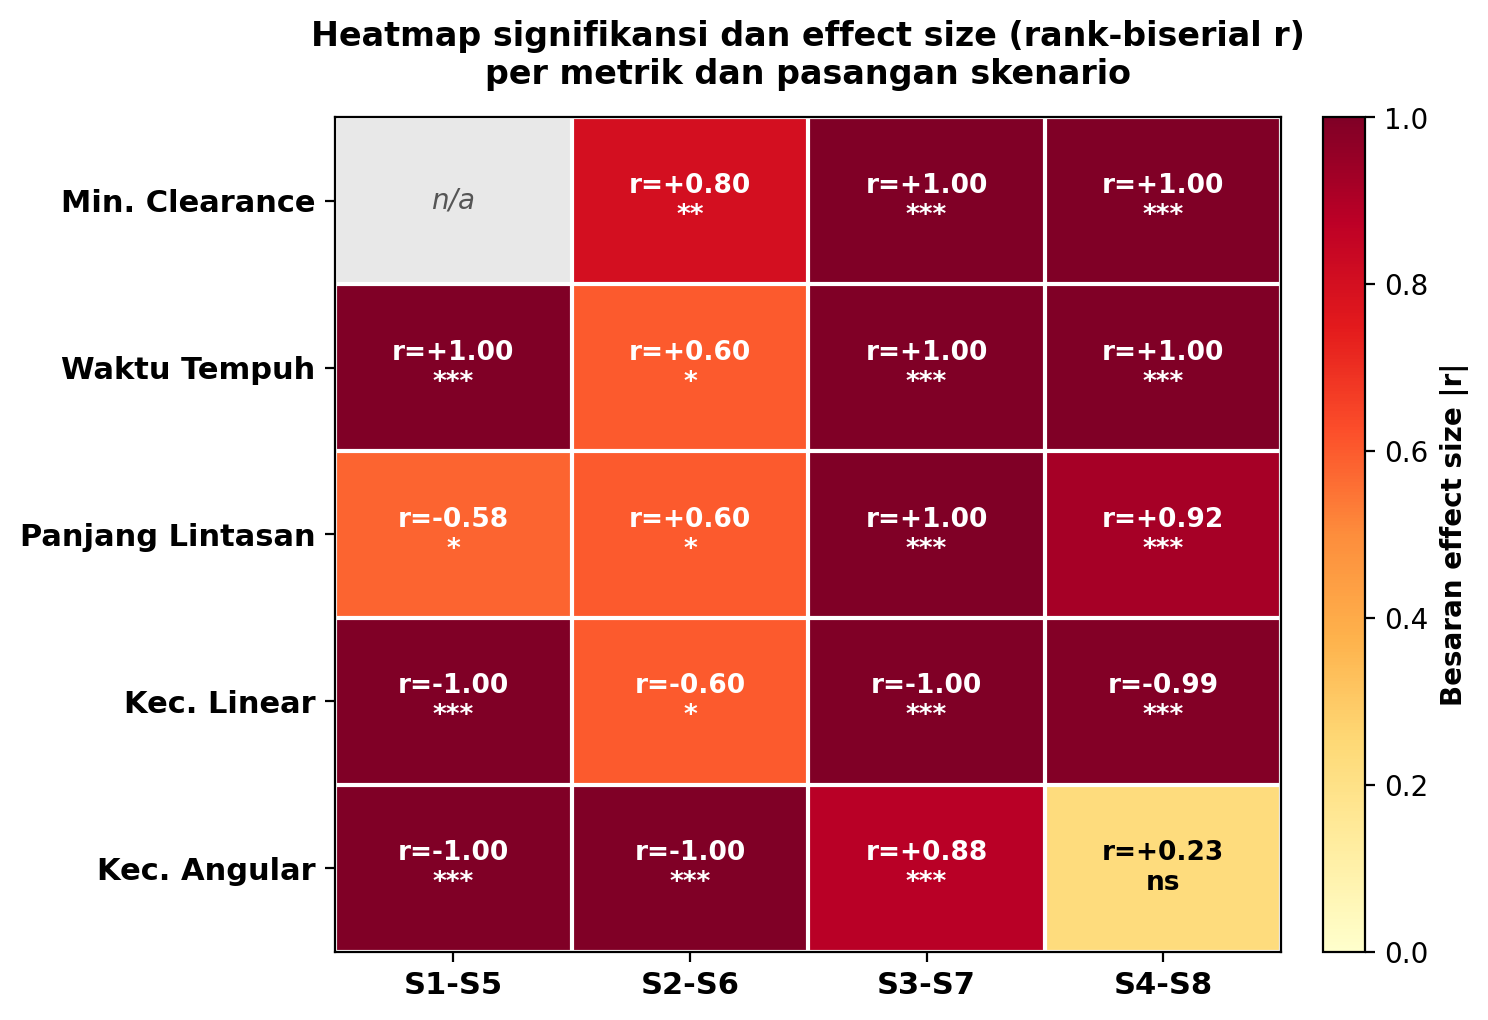
\includegraphics[width=0.92\textwidth]{gambar/4.7_heatmap_statistik.png}
\caption{Heatmap besaran effect size ($|r|$) dan signifikansi untuk seluruh
metrik kontinu pada keempat pasangan skenario. Warna menunjukkan besaran
$|r|$, anotasi menunjukkan nilai $r$ bertanda beserta simbol signifikansi.}
\label{fig:heatmap_statistik}
\end{figure}

Gambar~\ref{fig:heatmap_statistik} memperlihatkan pola di atas secara
visual: hampir seluruh sel berwarna gelap (effect size besar), dengan satu
sel pucat yang jelas berbeda, yaitu kecepatan angular pada S4/S8.

Dari sisi keselamatan, minimum clearance menunjukkan pola perubahan paling
konsisten di antara seluruh metrik yang diuji. Pada ketiga pasangan yang
dapat diuji, peningkatan clearance pada \textit{proposed method} selalu
signifikan dengan effect size besar, dan besarnya effect size ini
cenderung membesar seiring kompleksitas skenario, dari $r=+0,80$ pada
S2/S6 menjadi $r=+1,00$ pada S3/S7 dan S4/S8, skenario yang melibatkan
\textit{blind-spot} dan \textit{obstacle} dinamis.

Dari sisi efisiensi, waktu tempuh menunjukkan \textit{trade-off} yang juga
konsisten, signifikan pada keempat pasangan dengan effect size besar.
Namun, sebagaimana telah dibahas pada Subbab~\ref{sec:tradeoff}, effect
size besar tidak selalu sejalan dengan selisih absolut yang besar. Panjang
lintasan pada S1/S5 misalnya signifikan dengan effect size besar
($r=-0,58$), padahal selisih absolutnya hanya 0,01~m. Effect size pada
metrik efisiensi karena itu perlu dibaca berdampingan dengan selisih
absolut pada tabel-tabel deskriptif sebelumnya, bukan sebagai ukuran
tunggal kepentingan praktis.

Dari sisi kualitas gerak, perubahan pada kecepatan angular tidak menunjukkan
pola yang seragam seperti clearance. Signifikan dengan effect size besar
pada S1/S5, S2/S6, dan S3/S7, namun satu-satunya kombinasi tidak signifikan
pada keseluruhan penelitian ini justru ditemukan di sini, pada S4/S8.
Pola ini menunjukkan bahwa peningkatan keselamatan pada skenario dinamis
tidak selalu disertai perubahan kualitas gerak rata-rata yang sama
drastisnya, konsisten dengan temuan kualitatif pada
Subbab~\ref{sec:kehalusan_gerak} bahwa perbedaan pada pasangan ini lebih
terlihat dari sisi konsistensi antar-\textit{trial} dibanding kecepatan
angular rata-rata.

Secara terintegrasi, data di atas menjawab beberapa pertanyaan mendasar
secara hati-hati. Untuk metrik keselamatan, metode usulan secara statistik
teruji lebih aman dibandingkan \textit{baseline} pada seluruh skenario yang
melibatkan \textit{obstacle}, dengan effect size yang konsisten besar.
Peningkatan ini juga bermakna secara praktis terutama pada S3/S7 dan S4/S8,
tempat selisih absolut clearance mencapai puluhan sentimeter, dibandingkan
S2/S6 yang selisihnya hanya beberapa milimeter meski tetap signifikan.
Biaya efisiensi yang menyertainya, berupa kenaikan waktu tempuh 15,5\%
hingga 63,7\%, tergolong dapat diterima apabila prioritas utama aplikasi
adalah keselamatan, namun keputusan ini pada akhirnya bergantung pada
kebutuhan operasional spesifik dan tidak dapat digeneralisasi berlaku
untuk seluruh aplikasi. Manfaat metode usulan paling terlihat pada kondisi
yang melibatkan \textit{blind-spot} dan \textit{obstacle} dinamis (S3/S7
dan S4/S8), yaitu kondisi yang memang menjadi sasaran rancangan utama
penelitian ini, sementara pada kondisi sederhana seperti lingkungan terbuka
(S1/S5), manfaat keselamatan tidak relevan untuk dievaluasi karena memang
tidak ada \textit{obstacle} yang perlu dihindari.

Tujuan penelitian ini, yaitu meningkatkan keselamatan navigasi pada kondisi
\textit{blind-spot} sambil mempertahankan keberhasilan dan menjaga efisiensi
pada tingkat yang masih dapat diterima, secara umum didukung oleh hasil
statistik di atas. Peningkatan keselamatan teruji konsisten dan besar,
keberhasilan navigasi tetap terjaga pada hampir seluruh skenario
(Subbab~\ref{sec:keberhasilan_tabrakan}), dan biaya efisiensi yang
menyertainya terukur dan tidak berlebihan pada sebagian besar pasangan.
Meskipun demikian, hasil ini tidak dapat dibaca sebagai pembuktian mutlak
atas seluruh hipotesis penelitian, mengingat keterbatasan jumlah
\textit{trial} dan lingkup simulasi yang dibahas pada bagian berikut.

Beberapa keterbatasan perlu dipertimbangkan dalam membaca sintesis statistik
ini. Pertama, ukuran sampel pada setiap kelompok relatif kecil ($n=10$),
sehingga meskipun effect size telah dilaporkan untuk mengurangi risiko
salah tafsir akibat sampel kecil, estimasi presisi tetap terbatas. Kedua,
seluruh hasil diperoleh dari simulasi Gazebo yang belum sepenuhnya
merepresentasikan dinamika dunia nyata. Ketiga, penelitian ini tidak
melakukan \textit{ablation study}, sehingga kontribusi masing-masing
komponen metode usulan, virtual scan, fusi \textit{traversability}, dan
adaptasi fuzzy, terhadap hasil statistik di atas tidak dapat dipisahkan
satu sama lain.

Pembaca juga perlu mencermati bahwa signifikansi statistik tidak selalu
identik dengan relevansi praktis, sebagaimana telah ditunjukkan oleh kasus
panjang lintasan pada S1/S5. Effect size besar pada satu metrik tidak
otomatis berarti penting bagi seluruh aplikasi; bobot kepentingan setiap
metrik, apakah keselamatan lebih diutamakan dibanding efisiensi waktu,
pada akhirnya bergantung pada konteks penggunaan robot yang dituju, bukan
sesuatu yang dapat ditentukan semata dari hasil statistik ini.

Setelah hasil statistik disintesis secara menyeluruh pada subbab ini,
pembahasan berikutnya mengintegrasikan seluruh temuan, deskriptif,
statistik, dan kualitatif, untuk menjawab pertanyaan penelitian dan
mengevaluasi kontribusi metode usulan secara komprehensif pada
Subbab 4.8 Pembahasan Terintegrasi.